%!TEX root = ../thesis.tex
%*******************************************************************************
%****************************** Third Chapter **********************************
%*******************************************************************************
\chapter{Internal Magnetic Fields}

\section{Solar Magnetic Field}\label{mag_intro}

It is well known through the observation of much surface solar phenomenon like active regions, solar flares, coronal mass ejections etc, that the sun has in its interior, often highly localised, significant magnetic fields. The source of this magetic field is theorised to be a primordial current which started a dynamo process that is kept going at the expense of continous dissipation of energy from the solar bulk (CITE DYNAMO). It is also widely belived however that mean magnetic field throughout the solar bulk is fairly weak. This chapter is devoted to finding a method to observe signature of this magnetic field in the p-mode frequency spectrum.

Most of high intensity magnetic activity is limited to the solar surface. The tachocline is believed to contain toroidal fields as high as $10^5 \text{G}$ (CITE TACH). outside the tachocline the magnetic field is believed to be mostly dipolar such that mean surface magnetic field is about $10\text{G}$. Very strong local magnetic fields apart from these are also known to exist, but detection of such fields is outside the scope of this work; here we shall only investigate the effect of \textit{global} fields. It will be shown in this chapter why the method of frequency splittings is not the best way to detect strongly localised magentic fields.

\section{Equation of Motion}

In the presence of background magnetic field $\Bv$, the equation of motion is governed by the new operator $\cL \rightarrow \cL + \dL^{B}$, where $\dL^B$ is estabished in \cite{hanasoge17} as below.
\begin{align}
    \dLB \boldsymbol{\xi} &= \frac{-1}{4\pi}\boldsymbol{\nabla \cdot} [\Bv\Bv\cdot \boldsymbol{\nabla} \boldsymbol{\xi} + \Bv {\cdot} \boldsymbol{\nabla}\boldsymbol{\xi}\Bv - 2 \Bv\Bv\boldsymbol{\nabla \cdot}\boldsymbol{\xi} - (\boldsymbol{\xi \cdot \nabla} \Bv)\Bv - \Bv(\boldsymbol{\xi \cdot \nabla}\Bv)\notag
    \\& + B^2 \boldsymbol{\nabla \cdot \xi I} - \Bv\Bv :\boldsymbol{\nabla \xi I} + \boldsymbol{\xi \cdot \nabla}\frac{B^2}{2}\boldsymbol{I}] 
     \label{eqn: mag_pert_op}
\end{align}
where the $:$ stands for contraction of two second rank tensors ($\mathbf{P}:\mathbf{Q} \equiv P_{ij}Q_{ji} $).

Note that in above expression $\Bv$ only appears in the second order. This is a consequence of the induction equation where the Lagrangian displacement field $\xiv$ creates a current $\mathbf{j} \propto \xiv \times \Bv$ and this current interacts with magnetic field as $\mathbf{j} \times \Bv$ to give rise to acceleration. \cite{goedbloed2004} contains a detailed derivation of this and a proof of self adjointedness for $\dL^B$.

This expression can be put in a more convenient form involving the Lorentz stress tensor $\cH \equiv \Bv\Bv$ as
\begin{equation} \label{eqn: mag_pert_H}
    \dLB \boldsymbol{\xi} = \frac{-1}{4\pi}\boldsymbol{\nabla\cdot} [\boldsymbol{\mathcal{H}\cdot\nabla \xi} + (\boldsymbol{\nabla \xi})^T \boldsymbol{\cdot \mathcal{H}} - 2\boldsymbol{\mathcal{H}\nabla \cdot \xi} - \boldsymbol{\xi \cdot \nabla \mathcal{H}} + \boldsymbol{\mathcal{H}:I \nabla \cdot \xi I} - \cH{:}\boldsymbol{\nabla \xi I} + \boldsymbol{\xi \cdot \nabla} \enc{\frac{\cH{:}\boldsymbol{I}}{2}}\boldsymbol{I}]
\end{equation}

The tensor $\cH$ is the quantity of interest in this problem and any inversion algorithm must first invert splitting data for its components. It remains unclear if the magnetic field can be recovered from just the knowldge of components of $\cH$.

\section{Coupling Matrix}
\subsection{Lorentz Stress components}\label{sec:lorentz_stress_comps}
The process of taking integrals over a sphere becomes simplified if we're operating in the Generalised Sopherical Harmonics formalism. In this formalism (look at \ref{app_gsh} for basis of this formalism), magnetic field and Lorentz stress are decomposed as
$$\Bv = \sum_{st}\sum_{\alpha} B^{\alpha}_{st}(r) Y_{st}^{\alpha}(\theta,\phi) \ev{\alpha}$$
$$\cH = \sum_{st}\sum_{\mu\nu} h_{st}^{\mu\nu}(r) Y^{\mu+\nu}_{st}(\theta,\phi) \ev{\mu}\ev{\nu}$$
where the generalised spherical harmonic (GSH) coordinate indices given by Greek symbols run from $-1$ to $+1$.
It is not very productive to find general expressions relating $\Bv$ components to $\cH$ components. Instead, we'll find special relations pertaining to the kind of magnetic field at hand when necessary. $\cH$ by construction satisfies the symmetry property $h^{\mu\nu}_{st} = h^{\nu\mu}_{st}$ ($\because \cH = \Bv\Bv$), and $\enc{h^{\mu\nu}_{st}}^* = (-1)^t h_{s\bar{t}}^{\bar{\mu}\bar{\nu}}$, where overbars represent negatives, follows from its realness condition.

\subsection{Sensitivity Kernels}
Coupling matrix element is given as on integral transform over $\cH$ as
\begin{equation}\label{lor_kernel_intro}
\LamB_{k'k} = \inner{\xiv_{k'}}{\dLB\xiv_{k}}=\int_0^{R_{\odot}} dr r^2 \sum_{\substack{st \\ \mu\nu}} \cB_{st}^{\mu\nu}(r) h_{st}^{\mu\nu}(r)
\end{equation}
where $\cB_{st}^{\mu\nu}$ are the eigenfunction dependent magnetic sensitivity kernels. Prescription for evaluating these kernels and the explicit expressions can be found in \cite{hanasoge17}. It should be noted however that the coupling integral $\inner{\xiv_{k'}}{\dLB\xiv_{k}}$ can be reduced to the radial integral form obtained in  (\ref{lor_kernel_intro}) contains no boundary terms. It is indeed the case that the magnetic field is assumed to vanish at the surface in this analysis. Relaxing this assumption will introduce boundary terms which involve integrals only over the solar surface.
Since $h_{st}^{\mu\nu}$ is symmetric in interchange of $\mu$ and $\nu$, we may ascribe the same symmetry to $\cB_{st}^{\mu\nu}$ too without any loss in generality.

Using the Mathematica package developed for this work \cite{GSH_repo} which automates manipulation of tensor spherical harmonics via the method of GSHs, the following forms of the kernels were found

\begin{dmath}
\cB_{st}^{--} = \frac{(-1)^{m'+1}}{r^2}\gam{l}\gam{l'}\gam{s}\wigred{-m'}{t}{m} \enccrl{\wigred{1}{-2}{1}\om{l}{0}\om{l'}{0} \encsqr{\enc{U+{\om{l'}{2}}^2 V}V' - UU'-rV\dot{V}'} +\wigred{2}{-2}{0} \om{l'}{0}\om{l'}{2}\encsqr{(U+r\dot{U})V'-rU\dot{V}'} +\wigred{0}{-2}{2} \om{l}{0}\om{l}{2}rV\dot{U}' + \wigred{3}{-2}{-1} \om{l}{0}\om{l'}{0}\om{l'}{2}\om{l'}{3}VV'}   
\end{dmath}

\begin{dmath}
2\cB_{st}^{0-} = \frac{(-1)^{m'}}{r^2}\gam{l}\gam{l'}\gam{s}\wigred{-m'}{t}{m} \enccrl{\wigred{0}{-1}{1}\om{l}{0}\encsqr{\enc{2U+{\om{l'}{2}}^2 V}U' +{\om{l'}{0}}^2 \enc{-2UV'-VV'+rV\dot{V}'} -r\enc{U+V-r\dot{V}'}\dot{U}'} - \wigred{1}{-1}{0}\om{l'}{0}\encsqr{(-2U+{\om{l}{0}}^2V)U' + {\om{l}{0}}^2V\enc{r\dot{V}'-V'} + U\enc{2V' + r (\dot{U}' - 2\dot{V}' + r\ddot{V}')}}  +\wigred{-1}{-1}{2}\om{l}{0}\om{l'}{0}\om{l}{2}V\encsqr{U'-V'+r\dot{V}'} + \wigred{2}{-1}{-1}\om{l}{0} \om{l'}{0} \om{l'}{2}\encsqr{V\enc{U'-3V'+r\dot{V}'}+2r\dot{V}V'}} 
\end{dmath}

\begin{dmath}
\cB_{st}^{00} = \frac{(-1)^{m'}}{2r^2}\gam{l}\gam{l'}\gam{s}\wigred{-m'}{t}{m} \enccrl{-\encsqr{\wigred{-1}{0}{1}+\wigred{1}{0}{-1}}\om{l'}{0}\om{l}{0} \encsqr{V\enc{-4U'+2\enc{1+{\om{l'}{0}}^2} V'+r\enc{\dot{U}'-2\dot{V}'}} +2r\dot{V}\enc{U'-V'+r\dot{V}'}} +
\wigred{0}{0}{0}\encsqr{ \enc{6U-4{\om{l}{0}}^2 V-2 r \dot{U}} \enc{U'-{\om{l'}{0}}^2V'} + 2{\om{l'}{0}}^2 rU\dot{V}' + r\enc{\enc{-4U+2{\om{l}{0}}^2V+r\dot{U}}}\dot{U}'+rU\ddot{U}' }
} 
\end{dmath}

\begin{dmath}
\cB_{st}^{+-} = \frac{(-1)^{m'}}{2r^2}\gam{l}\gam{l'}\gam{s}\wigred{-m'}{t}{m} \enccrl{-2\encsqr{\wigred{-2}{0}{2}+\wigred{2}{0}{-2}} \om{l}{0}\om{l}{2} \om{l'}{0}\om{l'}{2} VV' + \wigred{-1}{0}{1}\om{l'}{0}\om{l}{0}\encsqr{-rV\dot{U}' + U \enc{U'-V'+r\dot{V}'}}}  
\end{dmath}

Kernel components $\cB_{st}^{\mu\nu}$ are found to have these following properties.
\begin{enumerate}
\item $\cB_{st}^{\mu\nu} = \cB_{st}^{\nu\mu}$ (by construction)
\item $\cB_{st}^{--} = (-1)^{l+l'+s}\cB_{st}^{++}$
\item $\cB_{st}^{0-} = (-1)^{l+l'+s}\cB_{st}^{+0}$
\item $\cB_{st}^{00} = \cB_{st}^{+-}=\cB_{st}^{-+}=0$ for odd $l'+l+s$
\end{enumerate}



\section{Synthetic Magnetic Field}
Using some basic pieces of information about mean solar magnetic field as given in \ref{mag_intro}, we can posit the following form of a synthetic magnetic field which will be used for validating our routine of finding frequency splits. We give the following form of the magnetic field which is comoposed of an internal toroidal field concentrated at the tachocline, and a dipolar field which entends from the tachocline to the surface.

\subsection{Construction of $\Bv$}\label{sec:B_construction}
Using the identities $\grad_1 Y_l^m = \om{l}{0} \enc{Y_{lm}^{-1} \ev{-} + Y_{lm}^0 \ev{+}}$, $\ev{r} \times\grad_1 Y_l^m = i\om{l}{0} \enc{Y_{lm}^{-1} \ev{-} - Y_{lm}^0 \ev{+}}$, and $Y_1^0(\theta,\phi) = \gam{1}\cos\theta$ we see following things: (1) A toroidal field $\Bv = \alpha(r) \sin\theta \ev{\phi}$ can be given as $B_{10} = i \alpha(r) / \gam{1} \enc{-1,0,1}$ with all other $B_{st}$ components being $0$, and (2) A dipolar field $\Bv = \beta(r) (2\cos\theta \ev{r} + \sin\theta\ev{\theta})$ with $\beta \propto r^{-3}$ can be given as $B_{10} = -\beta(r)/\gam{1} \enc{1,-2,1}$ with all other $B_{st}$ components being $0$. Note that the row vector refers to the GSH coordinate index $\mu$. This leads to the following final form of $\Bv$

\begin{equation}\label{mag_field}
B_{st}(r) = 
\begin{cases}
-i \frac{\alpha(r)}{\gam{1}} \gshvec{1}{0}{-1}  - \frac{\beta(r)}{\gam{1}} \gshvec{b-r\dot{b}}{-2b}{b-r\dot{b}}, & \text{for} (s,t) = (1,0) \\
0, & \text{for} (s,t) \neq (1,0)
\end{cases}
\end{equation}
where $b(r)=1$ where field is perfectly dipolar. The term $r\dot{b}(r)$ appear as a consequence of fixing the diveregence to zero and is only nonzero in the transition region where $b(r)$ goes from $0$ to $1$. It was can be checked via using $\grad \cdot \Bv = g_{\alpha\beta} (\grad\Bv)^{\alpha\beta}$ (\cite{GSH_repo} was used) that the two parts in (\ref{mag_field}) (toroidal and dipolar) satisfy the solenoidal condition independenlty. We plot the forms of the $\alpha$, $\beta$, and $b$ used in our frequency splitting calculations.

\begin{figure}[h]
\begin{subfigure}{0.5\linewidth}
\centering
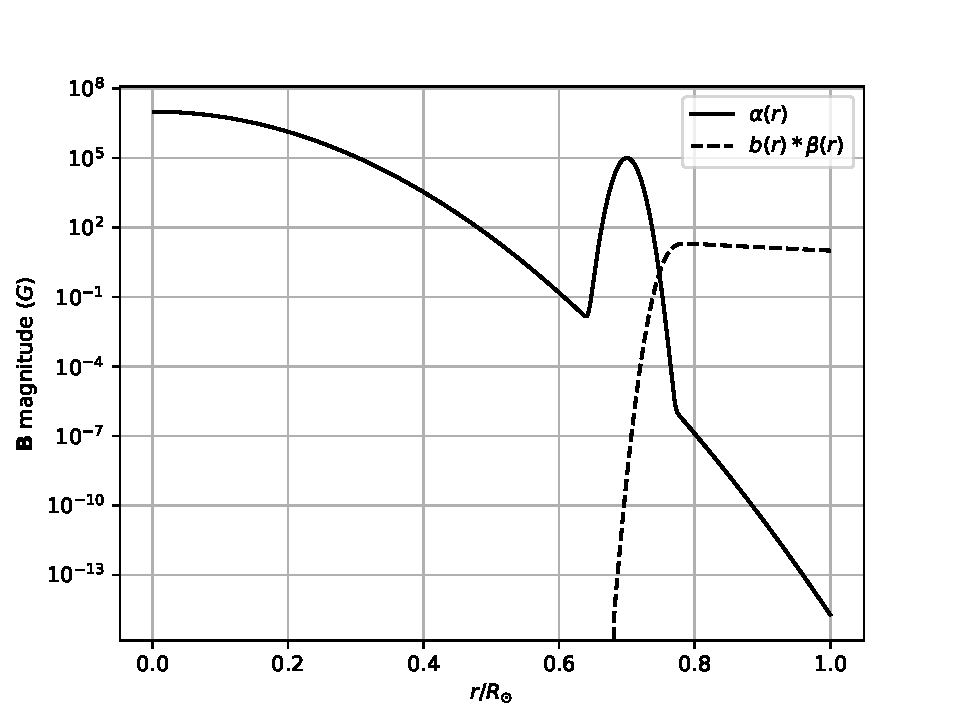
\includegraphics[scale=.5]{Chapter3/figs/alpha_beta}
\caption{$\alpha$ and $b * \beta$ in $G$}
\label{fig:alpha_beta}
\end{subfigure}
\begin{subfigure}{0.5\linewidth}
\centering
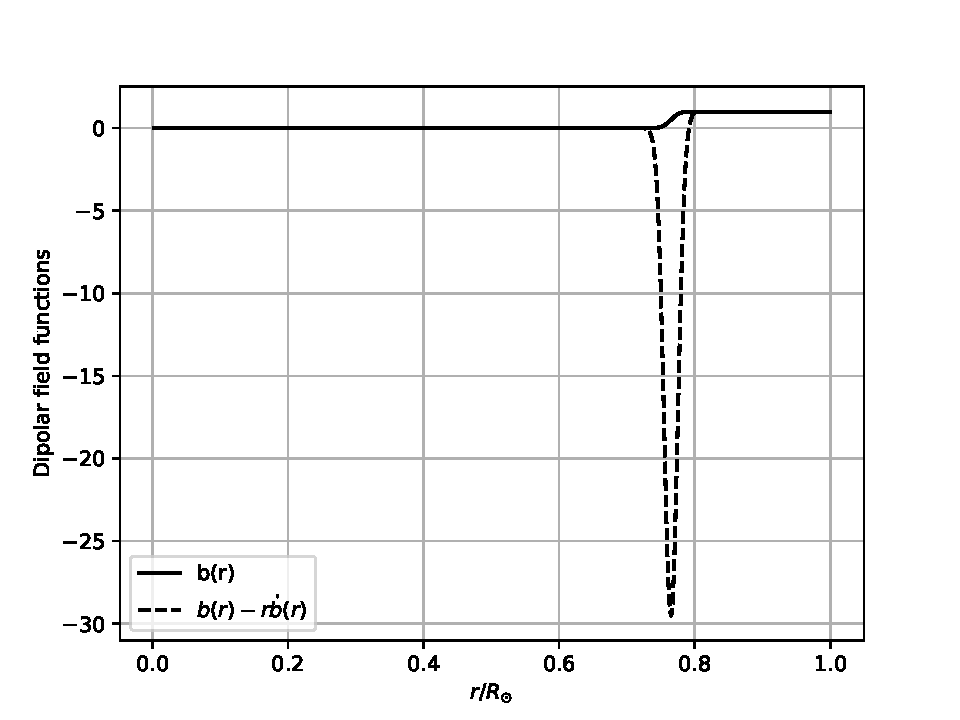
\includegraphics[scale=0.5]{Chapter3/figs/b}
\caption{$b$ and $a = b-r\dot{b}$}
\label{fig:a_b}
\end{subfigure}
\caption{$\alpha$ is addition of two Gaussians centred at $r=0$ with peak $10^7 G$ and at $r=0.7R_{\odot}$ with peak $10^5 G$ respectively. $b$ transitions smoothly from $0$ to $1$ as a sigmoid around $r=0.7R_{\odot}$. $r=0.7R_{\odot}$ mark is roughly where the tachocline is placed. Figure \ref{fig:alpha_beta} shows the poloidal (dipolar) field $\beta$ starting to dominate over the toroidal field by atleast three orders of magnitude as $r$ exceeds $\sim 0.8 R_{\odot}$.}
\end{figure}

\subsection{Construction of $\mathcal{H}$}

After the form of $\Bv$ has been ascertained, it is straighforward to derive components of $\cH$ via taking a tensor product. Decomposing either field in their GSH forms as in \ref{sec:lorentz_stress_comps}, and using orthonormality relation
\begin{equation}
\int d\Omega \enc{Y_{l_1m_1}^{n_1}}^*Y_{l_2m_2}^{n_2} = \delta_{l_1l_2}\delta_{m_1m_2}\delta_{N_1N_2}
\end{equation}

and the triple integral result

\begin{equation}\label{eq:triple_integral}
\int d\Omega \enc{Y_{l_1m_1}^{N_1}}^*Y_{l_2m_2}^{N_2}  Y_{l_3m_3}^{N_3}= (-1)^{m_1+N_1}4\pi \gam{l_1}\gam{l_2}\gam{l_3} \wigfull{l_1}{l_2}{l_3}{-m_1}{m_2}{m_3} \wigfull{l_1}{l_2}{l_3}{-N_1}{N_2}{N_3}
\end{equation}

one can write
\begin{equation}
h^{\mu\nu}_{st} = \sum_{\substack{s_1t_1\\ s_2t_2}} \langle Y_{st}^{\mu+\nu}, Y_{s_1 t_1}^{\mu}  Y_{s_2 t_2}^{\nu}\rangle B_{s_1t_1}^{\mu} B_{s_2t_2}^{\nu}
\end{equation}
Where $\langle Y_{l_1m_1}^{n_1}, Y_{l_2m_2}^{N_2}  Y_{l_3m_3}^{N_3}\rangle$ stands for the integral in eq(\ref{eq:triple_integral}).
If $\Bv$ has only $s=s_0$ and $t=t_0$ features, that is $\Bv = \sum_{\alpha}B_{s_0t_0}^{\alpha}Y_{s_0t_0}^{\alpha} \ev{\alpha}$, components of $\cH$ are given by
\begin{equation}\label{eq:single_feature_B}
h_{st}^{\mu\nu} = B^{\mu}_{s_0 t_0}B^{\nu}_{s_0 t_0} (-1)^{\mu + \nu + t} (2s_0+1) \gam{s} \wigfull{s_0}{s}{s_0}{\mu}{-(\mu+\nu)}{\nu} \wigfull{s_0}{s}{s_0}{t_0}{-t}{t_0}
\end{equation}

For the axis symmetric magnetic field constructed in \ref{sec:B_construction}, we may set $s_0=1$ and $t_0=0$. Wigner 3j selection rules given in \ref{sec:selec_rules} dicate that $\cH$ can only have $s=0,1,2$ and $t=0$. Then we have the form

\begin{equation}
h_{s0}^{\mu\nu} = 3 \gam{s} B^{\mu}_{10}B^{\nu}_{10} (-1)^{\mu + \nu} \wigfull{1}{s}{1}{\mu}{-(\mu+\nu)}{\nu} \wigfull{1}{s}{1}{0}{0}{0}
\end{equation}

But we know that $\wigfull{1}{s}{1}{0}{0}{0}$ vanishes for odd s. Thus we note here that $\cH$ has no $s=1$ and has non-zero $s=0$ components, which is different from how differential rotation couples modes. The $s=0$ feature of the Lorentz stress tensor indicates a net shift from the unperturbed mode frequency $\omega_{{nl}}$ for a particular multiplet $\mode{n}{l}$ as this term couples with $\wigfull{l'}{0}{l}{-m}{0}{m}$ which is independent of $m$.